\documentclass[oneside]{ctexbook}
\usepackage{graphicx}
\usepackage{amsmath}
\usepackage{xeCJK}
\usepackage{lmodern}
\usepackage{siunitx}
\usepackage{amssymb}
\usepackage{geometry}
\usepackage{amsfonts}
\usepackage{tikz}
\usepackage[toc]{multitoc}
\usepackage[colorlinks]{hyperref}
\geometry{a4paper,left=2.5cm,right=2.5cm,top=3cm,bottom=3cm}
\setlength{\headheight}{12.64723pt}
\addtolength{\topmargin}{-0.64723pt}
\setcounter{tocdepth}{1}
\linespread{1.8}\selectfont
\title{热力学}
\author{***}
\date{期末复习资料}
\begin{document}

\maketitle

教材《热力学与统计物理》,汪志诚,第六版

部分图片未画出,已经标注其在教材中的位置

\tableofcontents

\chapter{热力学的基本规律}

\section{热力学系统(教材P2)}
\begin{enumerate}
    \item \textbf{孤立系:}与外界既没有物质交换,也没有能量交换的系统。
    \item \textbf{封闭系统(闭系):}与外界没有物质交换,但是有能量交换。
    \item \textbf{开放系统(开系):}与外界既有物质交换,又有能量交换。
\end{enumerate}

\section{几个与物态方程有关的物理量(教材P7)}

\subsection{体胀参数}

在压强保持不变的条件下,温度升高1K所引起的物体体积的相对变化
\begin{equation}
\alpha=\dfrac{1}{V}\left(\dfrac{\partial{}V}{\partial{}T}\right)_p
\end{equation}

\subsection{压强系数}

在体积保持不变的条件下,温度升高1K所引起的物体压强的相对变化
\begin{equation}
\beta=\dfrac1p\left(\dfrac{\partial{}p}{\partial{}T}\right)_V
\end{equation}

\subsection{等温压缩系数}
在温度保持不变的条件下,增加单位压强所引起的物体体积的相对变化
\begin{equation}
\kappa_T=-\dfrac{1}{V}\left(\dfrac{\partial{}V}{\partial{p}}\right)_T
\end{equation}

\subsection{3个偏导数和3个系数之间的关系}
\begin{equation}
\left(\dfrac{\partial{}V}{\partial{p}}\right)_T\left(\dfrac{\partial{}p}{\partial{}T}\right)_V\left(\dfrac{\partial{}T}{\partial{}V}\right)_p=-1
\end{equation}

\begin{equation}
\alpha=\kappa_T\beta{}p
\end{equation}

注:这里偏微分括号外的下标表示该物理量视为不变的定值

\section{物态方程(教材P8)}

理想气体方程:\(PV=nRT\)

范德瓦尔斯方程(范德瓦尔斯气体所满足的方程):\((p+\dfrac{an^2}{V^2})(V-nb)=nRT\)

\section{热力学第零定律(热平衡定律)(教材P5)}

如果两物体A和B各自处于同一种状态的第三个物体C达到了热平衡,那么让A和B热接触后,A和B也将处于热平衡。(定义了温度)

\begin{figure}[h!]
    \centering
    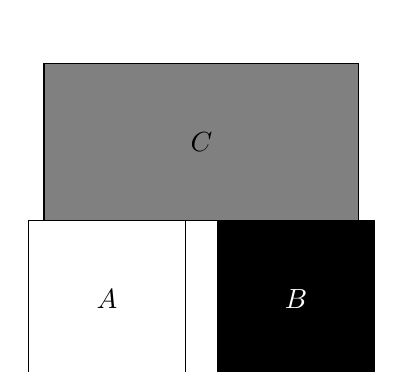
\begin{tikzpicture}
        \draw[fill=gray] (-2,0) rectangle node{\(C\)} (2,2);
        \draw (-2.2,-2) rectangle node{\(A\)} (-0.2,0);
        \draw[fill=black,text=white] (0.2,-2) rectangle node{\(B\)} (2.2,0);
    \end{tikzpicture}
    \hspace{2cm}
    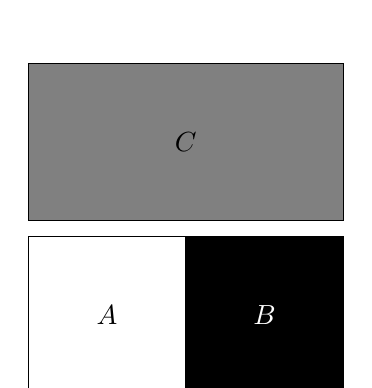
\begin{tikzpicture}
        \draw[fill=gray] (-2,0.2) rectangle node{\(C\)} (2,2.2);
        \draw (-2,-2) rectangle node{\(A\)} (0,0);
        \draw[fill=black,text=white] (0,-2) rectangle node{\(B\)} (2,0);
    \end{tikzpicture}
\end{figure}

\section{热力学第一定律(教材P17)}

自然界的一切物质都具有能量,能量有各种不同的形式,可以从一种形式转化为另一种形式,从一个物体传递到另一个物体。在传递与转化中,能量保持不变(即第一类永动机是不可能造成的)。

表达式:\(\mathrm{d}U=\delta{}Q+\delta{}W\)(内能的变化量等于系统从外界吸收的热量,与外界对系统做功之和)

补充:这里的W多指体积功,即\(W_{AB}=\int_A^Bp\mathrm{d}V\)。一般不考虑其他功。

\section{热力学第二定律(2种表述,教材P25)}
\begin{enumerate}
    \item \textbf{克劳修斯表述:}不可能把热量从低温物体传到高温物体而不引起其他变化。
    \item \textbf{开尔文表述:}不可能从单一热源吸热使之完全变成有用的功而不引起其他变化。
\end{enumerate}

注:两种表述彼此等价,表明热传导和功变热不可逆(方向性),即第二类永动机不可能实现。

不可逆过程列举:气体的自由膨胀过程,扩散过程,各种爆炸过程,墨水扩散,功变热,热传导,节流过程,焦耳实验的逆过程(气体自由膨胀)。

\section{热力学第三定律(教材P105-106)}
\begin{enumerate}
    \item \textbf{第一种表述:}凝聚系的熵在等温过程中改变随绝对温度趋于零。即:\begin{equation}\lim_{T\to{}0}(\Delta{}S)_T=0\end{equation}
    \item \textbf{第二种表述(绝对零度不能达到原理):}不可能使一个物体冷却到绝对零度。
\end{enumerate}

\section{热容(教材P17)}

\subsection{等容热熔\(C_V\)(体积不变,外界对系统不做功)}
\begin{equation}
C_V=\lim_{\Delta{}T\to0}\left(\dfrac{\Delta{}Q}{\Delta{}T}\right)_V=\lim_{\Delta{}T\to0}\left(\dfrac{\Delta{}U}{\Delta{}T}\right)_V=\left(\dfrac{\partial{}U}{\partial{}T}\right)_V
\end{equation}

\subsection{等压热容\(C_p\)(压强不变)}
\begin{gather*}
    C_p=\lim_{\Delta{}T\to0}\left(\dfrac{\Delta{}Q}{\Delta{}T}\right)_p=\lim_{\Delta{}T\to0}\left(\dfrac{\Delta{}U+p\Delta{}V}{\Delta{}T}\right)_p=\left(\dfrac{\partial{}U}{\partial{}T}\right)_p+p\left(\dfrac{\partial{}V}{\partial{}T}\right)_p\\
    H=U+pV
\end{gather*}

\subsection{理想气体满足\(C_p-C_V=nR\)(教材P19)}

对于理想气体,气体只要足够稀薄,分子间的平均距离足够大,相互作用的能量可以忽略,内能与体积无关。

因此,对于理想气体,偏导数可以写为导数,即
\begin{equation}
C_V=\dfrac{\mathrm{d}U}{\mathrm{d}T}
\end{equation}
\begin{equation}
U(T)-U_0=C_V\Delta{}T\text{(只要是理想气体就能求!)}
\end{equation}

将上式积分可以求出理想气体内能的积分表达式:
\begin{equation}
U=\int{}C_V\mathrm{d}T+U_0
\end{equation}

根据焓的定义式和理想气体的物态方程,可得理想气体的焓为:
\begin{equation}
H=U+pV=U+nRT
\end{equation}

\begin{center}
    (内能和焓在理想气体中,只是温度的函数)
\end{center}

说明理想气体的焓也只是温度的函数。因此,对于理想气体,偏导数也可以写成导数,即
\begin{equation}
C_p=\dfrac{\mathrm{d}H}{\mathrm{d}T}
\end{equation}

将上式积分,就可以得到理想气体焓的积分表达式:
\begin{equation}
H=\int{}C_p\mathrm{d}T+H_0
\end{equation}

由上式可得
\begin{equation}
C_p-C_V=nR
\end{equation}

上式给出理想气体的定压热容,和定容热容之差,引入绝热指数\(\gamma\),表示定压热容与定容热容的比值:
\begin{equation}
\gamma=\dfrac{C_p}{C_V}
\end{equation}

可将\(C_p\)和\(C_V\)用\(R\)和\(\gamma\)表示出来:
\begin{equation}
C_V=\dfrac{nR}{\gamma-1}\quad{}C_P=\gamma\dfrac{nR}{\gamma-1}
\end{equation}

\section{焓(教材P17)}
\begin{enumerate}
    \item \(H=U+pV\)(定义)
    \item \(\Delta{}H=\Delta{}U+p\Delta{}V\)(等压过程中焓的变化)
    \item \(\Delta{}H=\Delta{}U+\Delta{}(pV)\)(一般情况或者普遍情况)
\end{enumerate}

\section{焦耳定律}

虽然考试中没明确说明要考可是会考到
\begin{equation}
U=\dfrac{i}{2}nRT
\end{equation}

\begin{enumerate}
    \item 单原子分子\(i=3\)(考的最多)
    \item 双原子刚性分子\(i=5\)
    \item 双原子弹性分子\(i=6\)
\end{enumerate}

注:其中\(i\)为气体分子所具有的自由度

\section{卡诺循环(教材P22)}

以理想气体为工作物质,经历等温膨胀,绝热膨胀,等温压缩,绝热压缩4个准静态过程。

\subsection{热机(顺时针)(热机效率证明过程要会!)}

现在讨论理想气体的卡诺循环,考虑1mol理想气体进行下列四个准静态过程(考虑一切逆过程,这里都是绝对值,不带负号)。

\begin{figure}[htbp]%这个图有点草率,本来想用解析式画的,但是我懒。
    \centering
    \begin{tikzpicture}[>=latex]
        \node at (-0.2,-0.2){\(O\)};
        \draw[->](0,0)--(5,0)node[below]{\(V\)};
        \draw[->](0,0)--(0,5)node[left]{\(p\)};
        \draw(1,4)node[left]{\(I\)} to [bend right=5]node[above]{\(T_1\)} (3,3)node[above]{\(I\hspace{-0.1cm}I\)} to [bend right=5] (4,1) node[right]{\(I\hspace{-0.1cm}I\hspace{-0.1cm}I\)} to [bend left=5]node[below]{\(T_2\)} (2,2)node[left]{\(I\hspace{-0.08cm}V\)} to [bend left=5] cycle;
    \end{tikzpicture}
\end{figure}

\subsubsection{等温膨胀过程}%这个罗马数字是拼接出来的/TAT\

气体与温度为\(T_1\)的高温热源保持接触,从状态\(I(p_1,V_1,T_1)\)等温膨胀到状态\(I\hspace{-0.1cm}I(p_2,V_2,T_1)\)。在此过程中气体吸收的热量\(Q_1\)为:
\begin{equation}
Q_1=RT_1\ln\dfrac{V_2}{V_1}
\end{equation}

\subsubsection{绝热膨胀过程}

气体由状态\(I\hspace{-0.1cm}I(p_2,V_2,T_1)\)绝热膨胀到状态\(I\hspace{-0.1cm}I\hspace{-0.1cm}I(p_3,V_3,T_2)\)。在此过程中气体吸收的热量为零

\subsubsection{等温压缩过程}

气体与温度为\(T_2\)的高温热源保持接触,由状态\(I\hspace{-0.1cm}I\hspace{-0.1cm}I(p_3,V_3,T_2)\)等温压缩到状态\(I\hspace{-0.08cm}V(p_4,V_4,T_2)\)。在此过程中气体释放的热量\(Q_2\)为:
\begin{equation}
Q_2=RT_2\ln\dfrac{V_3}{V_4}
\end{equation}

\subsubsection{绝热压缩过程}

气体由状态\(I\hspace{-0.08cm}V(p_4,V_4,T_2)\)绝热压缩到状态\(I(p_1,V_1,T_1)\),在此过程中气体吸收的热量为零

\subsubsection{效率}

整个循环过程结束后,气体回到原来的状态,内能作为状态函数其变化为零。由热力学第一定律可知,在整个循环中气体对外做的净功应等于气体在循环过程中所吸收的净热量\(Q_1-Q_2\):
\begin{equation}
W=Q_1-Q_2=RT_1\ln\dfrac{V_2}{V_1}-RT_2\ln\dfrac{V_3}{V_4}
\end{equation}

此式可以化简,因为过程(二)和过程(四)是准静态过程,故有
\begin{equation*}
    \begin{aligned}
        T_1V_2^{\gamma-1}=T_2V_3^{\gamma-1}\\
        T_1V_1^{\gamma-1}=T_2V_4^{\gamma-1}
    \end{aligned}
\end{equation*}

从这两个方程消去\(T_1\)和\(T_2\),得
\begin{equation}
\dfrac{V_2}{V_1}=\dfrac{V_3}{V_4}
\end{equation}

因此
\begin{equation}
W=R(T_1-T_2)\ln\dfrac{V_2}{V_1}
\end{equation}

在这个循环中,气体从高温热源吸收了热量\(Q_1\),对外做功\(W\),故机械效率为
\begin{equation}
\eta=\dfrac{W}{Q_1}=\dfrac{R(T_1-T_2)\ln\dfrac{V_2}{V_1}}{RT_1\ln\dfrac{V_2}{V_1}}=1-\dfrac{T_2}{T_1}
\end{equation}

该效率恒小于1。原因是气体只把它从高温热源所吸取的热量的一部分转化为机械功,其余热量向低温热源放出去了。\(\eta\)给出的热功转化效率的大小只取决于两个热源的温度

\subsection{制冷机(逆时针)}

如果令整个循环反向进行,依次经\(I\to I\hspace{-0.08cm}V\to I\hspace{-0.1cm}I\hspace{-0.1cm}I\to I\hspace{-0.1cm}I\to I\),则由准静态过程逆过程的性质可知,在逆循环中外界对系统做功\(W=R(T_1-T_2)\ln\dfrac{V_2}{V_1}\),气体从低温热源\(T_2\)吸热\(Q_2=RT_2\ln\dfrac{V_3}{V_4}\)向高温热源\(T_1\)放热\(Q_1=RT_1\ln\dfrac{V_2}{V_1}\)。

这个逆循环是理想制冷机的工作循环,其作用是把热量从低温物体送到高温物体去。可以看出,在逆卡诺循环中,气体在把它从低温热源吸收的热量送到高温热源的同时,把外界对他所做的功也转化为热量送到高温热源去了。如果从低温热源吸取一定的热量\(Q_2\),所需外界的功越小,制冷机的性能就越好。所以我们可以定义制冷机的工作系数\(\eta{}'\),为从低温热源吸取的热量\(Q_2\)除以外界所做的功\(W\):
\begin{equation}
\eta{}'=\dfrac{Q_2}{W}
\end{equation}

根据前面的讨论,理想气体在逆卡诺循环中的工作系数等于
\begin{equation}
\eta{}'=\dfrac{T_2}{T_1-T_2}
\end{equation}

该工作系数也只取决与两个温度

补充:
\begin{enumerate}
    \item 准静态过程:系统的状态变化很缓慢,以至于过程中每一个状态都可以看做平衡态。
    \item 绝热过程:一个过程,其中系统状态的变换完全是由机械作用或者电磁作用的结果,而没有受到其他影响,称为绝热过程。
    \item 焦耳实验说明系统经绝热过程从初态到终态,在过程中外界对系统做的功取决于系统的初态和终态,而与具体绝热过程无关。
\end{enumerate}

总结:

热机:卡诺循环

制冷机:逆卡诺循环

\section{卡诺定理(教材P27)}

定义:所有工作于两个确定温度之间的热机,可逆热机的效率最高。

推论:所有工作于两个确定温度之间的可逆热机,其效率相等。

\section{克拉修斯不等式}
\begin{equation}
\dfrac{Q_1}{T_1}+\dfrac{Q_2}{T_2}\leq{}0
\end{equation}

注:
\begin{enumerate}
    \item \(Q_1\)是热机从\(T_1\)热源所吸收的热量,\(Q_2\)是热机从\(T_2\)热源所吸收的热量
    \item 不等式取等号时表明为可逆热机,取不等号时表明热机为不可逆热机
    \item 对于一个更普遍的循环过程,原式变为:\(\oint\dfrac{\delta{}Q}{T}\leq0\)
\end{enumerate}

\section{热力学温标(不怎么考,教材P28)}

\section{熵(教材P31)}
\begin{gather}
    S_B-S_A=\int_A^B\dfrac{\delta{}Q}{T}\label{熵定义}\\
    \mathrm{d}S=\dfrac{\delta{}Q}{T}=\dfrac{\mathrm{d}U+p\mathrm{d}V}{T}\notag\\
    \mathrm{d}U\leq{}T\mathrm{d}S-p\mathrm{d}V\notag
\end{gather}

\begin{center}
    (当且仅当过程可逆时取等号)
\end{center}

根据熵的广延性(熵时广延量)可将整个系统的熵定义为在局域平衡的各个部分的熵之和。

补充:
\begin{enumerate}
    \item \textbf{广延量:}与系统的质量或物质的量成正比的物理量,如\(m,V,S,U\)
    \item \textbf{强度量:}与系统的质量或物质的量无关的物理量,如\(p,T,\mu\)(化学势)
\end{enumerate}

\section{理想气体的熵(教材P33)}

\subsection{熵与等压热容}
\[S_m=\int\dfrac{C_{V,m}}{T}\mathrm{d}T+R\ln{}V_m+S_{m0}\]

在\(C_{V,m}\)可以看作常量的情况下,上式可以表示为:
\begin{equation}
\begin{aligned}
    S_m=C_{V,m}\ln{}T+R\ln{}V_m+S_{m0}\quad(1\mathrm{mol})\\
    S=nC_{V,m}\ln{}T+nR\ln{}V_m+S_{0}\quad(n\mathrm{mol})
\end{aligned}
\end{equation}

\subsection{熵与等容热容}
\[S_m=\int\dfrac{C_{p,m}}{T}\mathrm{d}T-R\ln{}p+S_{m0}\]

\begin{equation}
S_0=n(S_{m0}-R\ln{}p)%?
\end{equation}

在\(C_{p,m}\)可以看作常量时,有
\begin{gather*}
    S=nC_{p,m}\ln{}T-nR\ln{}p+S_0\quad(n\mathrm{mol})\\
    S_m=C_{p,m}\ln{}T-R\ln{}p+S_0\quad(1\mathrm{mol})\\
    S_0=nS_{m0}
\end{gather*}

注:这里的两个\(S_0\)是不相等的

\section{熵增加原理(教材P38)}

表述:在绝热状态下,熵减少的过程是不可能实现的。孤立系统中发生的不可逆过程,总是朝着混乱度增加的方向进行的。(即朝熵增加的方向进行,熵的末减初大于0)

注:
\begin{enumerate}
    \item 熵是系统中微观粒子无规则运动的混乱程度的定量表述。
    \item 熵增原理仅对绝热或孤立系统成立,而对非绝热过程不成立。
    \item 对绝热系或孤立系,可以通过\(\mathrm{d}S\)是否为0来判断过程是否可逆。
\end{enumerate}

计算熵的步骤:
\begin{enumerate}
    \item 选定系统
    \item 确定初末状态
    \item 任意构造一个可逆系统
    \item 计算熵增
\end{enumerate}

\begin{equation}
\Delta{}S=S_B-S_A=\int_A^B\dfrac{\delta{}Q}{T}
\end{equation}

\section{自由能(是等温等容系统的判据)(教材P38)}
\begin{enumerate}
    \item \(F=U-TS\)(定义式)
    \item \(-W\leq{}F_A-F_B\)(系统在等温过程中对外所做的功不大于其自由能的减小,即自由能的减小是在等温过程中从系统所能获得的最大功)
    \item 只有体积功的情况下,体积不变时\(W=0\),及\(F_B-F_A\leq{}0\)
\end{enumerate}

\section{吉布斯函数(是等温等压系统的判据)(教材P39)}
\begin{enumerate}
    \item \(G=F+pV=U-TS+pV\)
    \item \(G_B-G_A\leq{}0\)(在等温等压条件下,系统的吉布斯函数永不增加。在等温等压条件下,系统中发生的不可逆过程总是朝着吉布斯函数减小的方向进行的。)
\end{enumerate}

\chapter{均匀物质的热力学性质}

\section{内能,焓,自由能和吉布斯函数的全微分(教材P42)}
\begin{table}[h]
    \centering
    \begin{tabular}{ll}
        \(G=F+pV=U-TS+pV\)& \\
        \(H=U+pV\)&\(F=U-TS\) \\
        \(\mathrm{d}U=T\mathrm{d}S+p\mathrm{d}V\)&\(\mathrm{d}H=T\mathrm{d}S+V\mathrm{d}p\)\\
        \(\mathrm{d}F=-S\mathrm{d}T-p\mathrm{d}V\)&\(\mathrm{d}G=-S\mathrm{d}T+V\mathrm{d}p\)
    \end{tabular}
\end{table}

\section{麦克斯韦关系(教材P43)}
\begin{table}[h]
    \centering
    \begin{tabular}{cc}
        \(\left(\dfrac{\partial{}T}{\partial{}V}\right)_S=-\left(\dfrac{\partial{}p}{\partial{}S}\right)_V\)&\(\left(\dfrac{\partial{}T}{\partial{}p}\right)_S=\left(\dfrac{\partial{}V}{\partial{}S}\right)_p\)\\
        \(\left(\dfrac{\partial{}S}{\partial{}V}\right)_T=\left(\dfrac{\partial{}p}{\partial{}T}\right)_V\)&\(\left(\dfrac{\partial{}S}{\partial{}p}\right)_T=-\left(\dfrac{\partial{}V}{\partial{}T}\right)_p\) 
\end{tabular}
\end{table}

熟记口诀:开着SUV去哈佛和排骨汤。
\begin{table}[h]
    \centering
    \begin{tabular}{|c|c|c|}
        \hline
        S&U&V(-)\\
        \hline
        H&&F\\
        \hline
        P&G&T(-)\\
        \hline
    \end{tabular}
\end{table}

注:
\begin{enumerate}
    \item 左右对称,上下对称,当V对应于T的时候注意加-号。要求ST配对,PV配对
    \item 在横竖两个方向上的3个物理量的中间一个物理量的微分能用另外两个物理量作为自变量来表示。
\end{enumerate}

\begin{equation}
\begin{aligned}
    &\mathrm{d}U=T\mathrm{d}S-p\mathrm{d}V&\mathrm{d}H=T\mathrm{d}S+V\mathrm{d}p\\
    &\mathrm{d}F=-S\mathrm{d}T-p\mathrm{d}V&\mathrm{d}G=-S\mathrm{d}T+V\mathrm{d}p
\end{aligned}
\end{equation}

补充:
\begin{enumerate}
    \item 主要热力学函数:\(U,H,F,G,S\)和物态方程。
    \item 其中\(U,S\)和物态方程为基本热力学函数,其他热力学函数均可由它们导出。
    \item \(T,p,V\)为状态参量(即自变量)。
    \item 特性函数:适当选择独立变量,只用一个热力学函数就能推导得其他热力学函数,从而确定系数的全部热力学性质。特性函数必须与相应的特征变量配套使用。应用最广泛的特性函数是自由能和吉布斯函数。
\end{enumerate}

\begin{equation}
U=F-T\left(\dfrac{\partial{}F}{\partial{}T}\right)\quad{}H=G-T\left(\dfrac{\partial{}G}{\partial{}T}\right)
\end{equation}

\section{麦克斯韦关系的应用(能态与焓态关系)(教材P43-45)}
\begin{enumerate}
    \item \(\left(\dfrac{\partial{}U}{\partial{}V}\right)_T=T\left(\dfrac{\partial{}p}{\partial{}T}\right)_V-p\)(能态关系:在温度保持不变时内能随体积的变化率于物态方程的关系)\label{能态关系}
    \item \(\left(\dfrac{\partial{}H}{\partial{}p}\right)_T=V-T\left(\dfrac{\partial{}V}{\partial{}T}\right)_p\)(焓态关系:在温度保持不变时焓随压强的变化率与物态方程的关系)\label{焓态关系}
    \item 热容:\(C_V=\left(\dfrac{\partial{}U}{\partial{}T}\right)_V=T\left(\dfrac{\partial{}S}{\partial{}T}\right)_V\quad{}C_p=\left(\dfrac{\partial{}H}{\partial{}T}\right)_p=T\left(\dfrac{\partial{}S}{\partial{}T}\right)_p\)
    \item 两个热容之间的关系:\(C_p-C_V=T\left(\dfrac{\partial{}S}{\partial{}V}\right)_T\left(\dfrac{\partial{}V}{\partial{}T}\right)_p=T\left(\dfrac{\partial{}p}{\partial{}T}\right)_V\left(\dfrac{\partial{}V}{\partial{}T}\right)_p=\dfrac{VT\alpha^2}{\kappa_T}\)对于理想气体:\(C_p-C_V=nR\)
\end{enumerate}

补充:\ref{能态关系}和\ref{焓态关系}要会证明!(详见教材P44-45)

\section{雅可比行列式(教材P294-295)}

雅可比行列式是热力学中进行导数变换的一个有用的工具。设\(u,v\)是独立变量\(x,y\)的函数\(u=u(x,y),v=v(x,y)\)

雅可比行列式的定义是
\begin{equation}
\dfrac{\partial(u,v)}{\partial{}(x,y)}=\begin{vmatrix}
\dfrac{\partial{}u}{\partial{}x}&\dfrac{\partial{}u}{\partial{}y}\\
    \dfrac{\partial{}v}{\partial{}x}&\dfrac{\partial{}v}{\partial{}y}\\
    \end{vmatrix}=\dfrac{\partial{}u}{\partial{}x}\dfrac{\partial{}v}{\partial{}y}-\dfrac{\partial{}u}{\partial{}y}\dfrac{\partial{}v}{\partial{}x}
\end{equation}

下面列出雅可比行列式的几个性质
\begin{gather*}
    \left(\dfrac{\partial{}u}{\partial{}x}\right)_y=\dfrac{\partial(u,y)}{\partial{}(x,y)}\\
    \dfrac{\partial(u,v)}{\partial{}(x,y)}=-\dfrac{\partial(v,u)}{\partial{}(x,y)}=\dfrac{\partial(v,u)}{\partial{}(y,x)}\\
    \dfrac{\partial(u,v)}{\partial{}(x,y)}=\dfrac{\partial(u,v)}{\partial{}(r,s)}\dfrac{\partial(r,s)}{\partial{}(x,y)}\\
    \dfrac{\partial(u,v)}{\partial{}(x,y)}=1/\dfrac{\partial(x,y)}{\partial{}(u,v)}
\end{gather*}

注:一个偏微分的数学关系

对于\(S(T,p)=S[T,V(T,p)]\),有:\(\left(\dfrac{\partial{}S}{\partial{}T}\right)_p=\left(\dfrac{\partial{}S}{\partial{}T}\right)_V+\left(\dfrac{\partial{}S}{\partial{}V}\right)_T\left(\dfrac{\partial{}V}{\partial{}T}\right)_p\)

\section{气温的节流过程(教材P46)}

\subsection{气流节流的特点}
\begin{enumerate}
    \item 节流过程不可逆
    \item 节流前后焓不变
    \item 焦汤效应:气流节流前后温度改变
\end{enumerate}

\subsection{焦汤系数(焦耳——汤姆孙系数,教材P47)}
\begin{equation}
\mu=\left(\dfrac{\partial{}T}{\partial{}p}\right)_H=\dfrac{1}{C_p}\left[T\left(\dfrac{\partial{}V}{\partial{}T}\right)_p-V\right]=\dfrac{V}{C_p}(T\alpha-1)
\end{equation}

\(T\alpha>1\)即\(\mu>0\)即制冷:\(T\alpha<1\)即\(\mu<0\)即制热。

\subsection{理想气体在节流前后温度不变}

理想气体的内能只是温度的函数

\section{绝热膨胀过程(教材P49)}
\begin{enumerate}
    \item 理想气体自由绝热膨胀后温度不变,范氏气体绝热膨胀后温度降低
    \item \(\left(\dfrac{\partial{}T}{\partial{}p}\right)_S=\dfrac{T}{C_p}\left(\dfrac{\partial{}V}{\partial{}T}\right)_p=\dfrac{VT\alpha}{C_p}\)
\end{enumerate}

\section{内能的积分表达式(教材P49)}
\begin{equation}
U=\int\left\lbrace{}C_V\mathrm{d}T+\left[T\left(\dfrac{\partial{}p}{\partial{}T}\right)_V-p\right]\mathrm{d}V\right\rbrace+U_0
\end{equation}

\section{熵的积分表达式(教材P49-50)}
\begin{equation}
\begin{aligned}
    S&=\int\left\lbrace{}\dfrac{C_V}{T}\mathrm{d}T+\left(\dfrac{\partial{}p}{\partial{}T}\right)_V\mathrm{d}V\right\rbrace+S_0\\
    S&=\int\left\lbrace{}\dfrac{C_p}{T}\mathrm{d}T+\left(\dfrac{\partial{}V}{\partial{}T}\right)_p\mathrm{d}p\right\rbrace+S_0
\end{aligned}
\end{equation}

\chapter{单元系的相变}

\section{平衡判据(教材P63-64)}

\subsubsection{熵判据(等容等内能)——基本判据}

孤立系统达到平衡状态时,熵达到最大值,任何一个偏离此状态的小变动,都将使系统熵减小。

孤立系统处在平衡状态的充分必要条件:\(\Delta{}S<0\)

平衡时熵达到极大值,此时的平衡状态:\(\delta{}S=0\)

稳定性条件\(\delta{}^2S<0\)

(两个条件要同时满足)

\subsubsection{自由能判据(等温等容过程)}

在等温等容条件下,系统的自由能水平永不增加。平衡状态时,自由能达到最小值,任何一个偏离此状态的小变动,都将使系统的自由能增加。

与熵判据同理!

等温等容系统处在稳定平衡状态的充分必要条件:\(\Delta{}F>0\)

平衡条件\(\delta{}F=0\)

稳定条件\(\delta{}^2F>0\)

\subsection{吉布斯函数判据(等温等压过程)}

在等温等压条件下,系统的吉布斯函数永不增加。平衡状态时,吉布斯函数达到最小值,任何一个偏离的此状态的小变动,都将使系统的吉布斯函数增加。

等温等压系统处在稳定平衡状态的充分必要条件:\(\Delta{}G>0\)

平衡条件\(\delta{}G=0\)

稳定条件\(\delta{}^2G>0\)

\subsection{焓判据(等熵等压过程)}

在等温等压条件下,系统的焓永不增加。

平衡条件\(\delta{}H=0\)

稳定条件\(\delta{}^2H>0\)

\section{系统的平衡状态(教材P64)}

由系统(下标为0)和子系统(下标为1)构成的孤立系达到平衡时满足:
\begin{equation}
T_1=T_0,p_1=p_0
\end{equation}

结论:达到平衡时整个系统的温度和压强处处相等(均匀)。

\section{系统稳定性的平衡条件(教材P65-66)}
\begin{equation}
C_V>0,\left(\dfrac{\partial{}p}{\partial{}V}\right)_T<0\text{(平衡的稳定性条件)}
\end{equation}

说明:
\begin{enumerate}
    \item 当子系统的\(T\)高于媒介时,热量从子系统传向媒介,而\(C_V>0\)使子系统的温度降低,恢复平衡。
    \item 当子系统的\(p\)高于媒介时,子系统的体积增大,而\(\left(\dfrac{\partial{}p}{\partial{}V}\right)_T<0\),使得子系统的压强降低,恢复平衡。
\end{enumerate}

\section{部分概念(书上没有,这里归纳一下)}
\begin{enumerate}
    \item 单元系:只含一种化学组分的化学纯物质系统。例如\(\mathrm{O}_2,\mathrm{H}_2,\mathrm{H}_2\mathrm{O}\)等。
    \item 多元系:含有两种以上化学组分的系统。例如多种气体的混合气体。
    \item 相:系统中物理性质均匀分布的部分。
    \item 单相系(均匀系):一个系统的各个部分的(物理和化学)性质完全一样。
    \item 复相系:若一个系统不均匀,但可分为几个均匀的部分
    \item 相变:由一个相转变为另一个相。
    \item 单元复相系:只含有一种化学组分,多个相共存的系统。例如:冰,水,水蒸气(单元三项系)和未饱和的盐水溶液(二元单相系)。
\end{enumerate}

说明:
\begin{enumerate}
    \item 每一个相的平衡态由自身的状态参量表示,热力学函数为自身的状态参量的函数
    \item 各相之间的物质可以发生转移,故每一相可以视为开系
    \item 平衡时,各相之间存在约束
\end{enumerate}

\section{化学势(教材P67)}
\begin{equation}
\mu=\left(\dfrac{\partial{}G}{\partial{}n}\right)_{T,p}=G_m
\end{equation}

称为化学势,它等于在温度和压强保持不变的条件下,增加1mol物质时吉布斯函数的增量(化学势等于摩尔吉布斯函数,为强度量)。
\begin{equation}
\mathrm{d}G=-S\mathrm{d}T+V\mathrm{d}p+\mu\mathrm{d}n
\end{equation}

可得
\begin{equation}
S=-\left(\dfrac{\partial{}G}{\partial{}T}\right)_{p,n},V=\left(\dfrac{\partial{}G}{\partial{}p}\right)_{T,n},\mu=\left(\dfrac{\partial{}G}{\partial{}n}\right)_{T,p}
\end{equation}

\section{开系的内能,焓,自由能(教材P67)}
\begin{gather*}
    \mathrm{d}U=T\mathrm{d}S-p\mathrm{d}V+\mu\mathrm{d}n\\
    \mathrm{d}H=T\mathrm{d}S+V\mathrm{d}p+\mu\mathrm{d}n\\
    \mathrm{d}F=-S\mathrm{d}T-p\mathrm{d}V+\mu\mathrm{d}n
\end{gather*}

注:其实就是在闭系的基础上再加一个化学势相关的微分即可

\section{巨热力势(教材P67)}

定义:\(J=F-\mu{}n\)
\begin{equation}
\mathrm{d}J=-S\mathrm{d}T-p\mathrm{d}V-n\mathrm{d}\mu\text{(全微分形式)}
\end{equation}

\(J\)是以\(F,V,\mu\)为独立变量的特性函数
\begin{equation}
J=F-G=-pV
\end{equation}

\section{单元系的复相平衡条件(教材P68-69)}
\begin{enumerate}
    \item 热平衡条件\(T^\alpha=T^\beta\)
    \item 力学平衡条件\(p^\alpha=p^\beta\)
    \item 相变平衡条件\(\mu^\alpha=\mu^\beta\)
    \item 整个系统达到平衡时,两相的温度,压强和化学势必须分布相等,这就是单元复相系达到平衡所需要满足的条件。
\end{enumerate}

\section{扰动趋势(教材P69)}
\begin{enumerate}
    \item 热平衡方向:能量从高温的相传向低温的相。
    \item 力学平衡方向:压强大的相膨胀,压强小的相压缩。
    \item 相变平衡方向:物质从化学势高的地方转移到化学势低的相中去。(化学势的物理意义反映了物质从一种相向另一种相转变的能力。)
\end{enumerate}

\section{单元复相系的相图(教材P69)}
\begin{figure}[htbp]
    \centering%也许我不应该在这里使用其他颜色
    \begin{tikzpicture}[>=latex,scale=1.2]        
        \draw (0,0) to [bend right=10] node[fill=white]{升华线}(1,1) to [bend right=10] node[fill=white]{汽化线}(4,2)node[right]{\(C\)}node[above=3pt]{临界点};
        \draw (1,1) to [bend right=5] node[fill=white]{熔化线}(2,4);
        \draw[->] (0.5,1.5)node[above]{三相点} to (0.9,1.1);
        \node at (0.5,3){固};
        \node at (3,3){液};
        \node at (3,0.5){气};
        \fill[red] (1,1) circle (2pt);
        \fill[green] (4,2) circle (2pt);
        \node at (-0.2,-0.2){\(O\)};
        \draw[->](0,0)--(5,0)node[below]{\(T\)};
        \draw[->](0,0)--(0,5)node[left]{\(p\)};
    \end{tikzpicture}
\end{figure}

\subsection{“三线两点”}

三线:升华线(固体变为气体),熔化线(固体变为液体),汽化线(液体变成气体)。

两点:三相点(固液气三相共存),临界点\(C\)(液相全部汽化,此时汽化线中断)。

\subsection{相图(P-T图)}

其平衡态是在一定的温度和压强下的,根据吉布斯平衡判据,此时的吉布斯函数最小。

平衡相变:指系统物质从一个相转变为另一个相时,始终保持平衡状态。

二相共存条件:
\begin{equation}
    T^\alpha=T^\beta=T,p^\alpha=p^\beta=p,\mu^\alpha(T,p)=\mu^\beta(T,p)\label{二相共存条件}
\end{equation}

注:二相平衡中\(T\)和\(p\)只有一个独立改变。

三相共存条件:
\begin{equation}
T^\alpha=T^\beta=T^\gamma=T,p^\alpha=p^\beta=p^\gamma=p,\mu^\alpha(T,p)=\mu^\beta(T,p)=\mu^\gamma(T,p)
\end{equation}

注:三相平衡中\(T\)和\(p\)唯一确定。

\section{克拉伯龙方程(教材P71-72)}

\subsection{相变潜热\(L\)}

表示1mol物质从\(\alpha\)相变到\(\beta\)相所吸收的热量。
\begin{equation}
L=T(S_m^\beta-S_m^\alpha)
\end{equation}

\subsection{证明过程}

如果已知两相的化学势的表达式,由式\ref{二相共存条件}即可确定相图的两相平衡曲线。由于缺乏化学势的全部知识,实际上相图上的平衡曲线是由实验直接测定的。不过,根据热力学理论可以求出两相平衡曲线的斜率,设\((T,p)\),和\((T+\mathrm{d}T,p+\mathrm{d}p)\)是两相平衡曲线上临近的两点,如图\ref{pic:a}所示。在这两点上,两相的化学势都相等:

\begin{figure}[htbp]
    \centering
    \begin{tikzpicture}[>=latex]
        \node at (-0.2,-0.2){\(O\)};
        \draw[->](0,0)--(5,0)node[below]{\(T\)};
        \draw[->](0,0)--(0,3)node[left]{\(p\)};
        \draw (0.5,0.5) parabola (2.5,2.5);
        \fill (1.5,1)node[left]{\((T,p)\)} circle (1pt);
        \fill (1.7,1.22)node[right]{\((T+\mathrm{d}T,p+\mathrm{d}p)\)} circle (1pt);        
    \end{tikzpicture}
    \caption{克拉伯龙方程}\label{pic:a}
\end{figure}
\begin{gather*}
    \mu^\alpha(T,p)=\mu^\beta(T,p)\\
    \mu^\alpha(T+\mathrm{d}T,p+\mathrm{d}p)=\mu^\beta(T+\mathrm{d}T,p+\mathrm{d}p)
\end{gather*}

两式相减,得
\begin{equation}
    \mathrm{d}\mu^\alpha=\mathrm{d}\mu^\beta\label{微分相等}
\end{equation}

式\ref{微分相等}表示,当沿着平衡曲线由\((T,p)\)变到\((T+\mathrm{d}T,p+\mathrm{d}p)\)时,两相的化学势的变化相等。

化学势的全微分为:
\begin{equation}
\mathrm{d}\mu=-S_m\mathrm{d}T+V_m\mathrm{d}p
\end{equation}

其中\(S_m\)和\(V_m\)分别是摩尔熵和摩尔体积。代入式子\ref{微分相等}得
\begin{equation}
-S_m^\alpha\mathrm{d}T+V_m^\alpha\mathrm{d}p=-S_m^\beta\mathrm{d}T+V_m^\beta\mathrm{d}p
\end{equation}

或
\begin{equation}
    \dfrac{\mathrm{d}p}{\mathrm{d}T}=\dfrac{S_m^\beta-S_m^\alpha}{V_m^\beta-V_m^\alpha}\label{微商形式}
\end{equation}

以\(L\)表示1mol物质\(\alpha\)相转变到\(\beta\)相是所吸收的相变潜热,因为相变时物质的温度不变,由式\ref{熵定义}得
\begin{equation}
L=T(S_m^\alpha-S_m^\beta)
\end{equation}

带入式\ref{微商形式}得:
\begin{equation}
\dfrac{\mathrm{d}p}{\mathrm{d}T}=\dfrac{L}{T(V_m^\beta-V_m^\alpha)}
\end{equation}

\section{临界点和气液两相的转变(教材P73)}

\subsection{等温线图}

教材图3.5.1%这个图太难画了aaaaa
\begin{enumerate}
    \item 左图为高温下\(\mathrm{CO_2}\)的等温线。
    \item 临界温度\qty{31.1}{\degreeCelsius}以上为气相温度线。
    \item 临界温度可以分为3段\\左边 段几乎与\(p\)轴平行的为液相,右边段为气相,中间与\(v\)平行的为气液共存状态。此段随温度的升高而缩短。
    \item 临界温度时物质处于气液不分的状态。高于此温度时,液相不可能存在,物质都处于气相。临界点:\(\left(\dfrac{\partial{}p}{\partial{}V}\right)_T=0\)。
\end{enumerate}

\subsection{范式气体的等温线(教材P73-74)}

教材图3.5.2
\begin{gather*}
    \left(p+\dfrac{a}{v_m^2}\right)(V_m-b)=RT\\
    \Rightarrow{}p=\dfrac{RT}{V_m-b}-\dfrac{a}{V_m^2}
\end{gather*}

特点:
\begin{enumerate}
    \item 当\(T>T_C\),曲线类似于理想气体等温线(双曲线)。
    \item 当\(T=T_C\),曲线在\(C\)点处有一拐点。
    \item 当\(T<T_C\),曲线的中段有一极小值点\(J\)和一极大值点\(N\)。曲线\(JDN\)的斜率大于零。可以知道\(\left(\dfrac{\partial{}p}{\partial{}V_m}\right)_T>0\)
\end{enumerate}
\subsection{麦克斯韦等面积法则(教材P74)}

教材图3.5.3和3.5.4

对等温线上的两个状态\(p,p_0\)而言
\begin{equation}
\begin{aligned}
    &\because\mathrm{d}\mu=-S_m\mathrm{d}T+V_m\mathrm{d}p\\
    &\therefore\mu-\mu_0=\int_{p_0}^pV_m\mathrm{d}p
\end{aligned}
\end{equation}

根据等温等压下的吉布斯函数最小的要求(注:\(\mu\)是1mol吉布斯函数),可知\(\mu-p\)位图中折线\(OKBAMR\)上各点才代表系统的稳定平衡状态。

\(A,B\)两点为\(\mu-p\)图上同一点,根据\(\mu=\mu(T,p)\Rightarrow{}\mu_A=\mu_B\)
\begin{equation}
\mu_A-\mu_B=\int_{BNDA}V_m\mathrm{d}p=0
\end{equation}

面积\(BND=\)面积\(DJA\)——麦克斯韦等面积法则

注:直线\(BA\)为实际等温线

\section*{补充:临界点}

在\(T=T_C\)的等温线上有一点\(C\),它是这条曲线的拐点
\begin{equation}
\left(\dfrac{\partial{}p}{\partial{}V_m}\right)_T=0,\left(\dfrac{\partial^2p}{\partial{}V_m^2}\right)_T=0,\left(p+\dfrac{a}{v_m^2}\right)(V_m-b)=RT
\end{equation}

可求得临界温度\(T_C\),临界压强\(P_C\),临界体积\(V_{mC}\)
\begin{equation}
T_C=\dfrac{8a}{27Rb},P_C=\dfrac{a}{27b^2},V_{mC}=3b
\end{equation}

\(T_C\),\(P_C\)和\(V_{mC}\)之间的关系
\begin{equation}
\dfrac{RT_C}{P_CV_{mC}}=\dfrac{8}{3}=2.667\text{——称为临界系数}
\end{equation}

以\(T_C\),\(P_C\)和\(V_{mC}\)作为测量温度,压强和体积的单位,引入三个无量纲变量(对比温度,对比压强和对比体积)。
\begin{equation}
\begin{aligned}
    t^*=\dfrac{T}{T_C},p^*=\dfrac{p}{p_C},v^*=\dfrac{V_m}{V_{mC}}\\
    \Rightarrow{}\left(p^*+\dfrac{3}{v^{*2}}\right)\left(v^*-\dfrac{1}{3}\right)=\dfrac{8}{3}t^*
\end{aligned}
\end{equation}

最后一行方程被称为范氏对比方程(了解即可)

对比态定律:一切物质在相同对比温度和对比压强下,都有相同的对比体积,即采用对比变量,各种气体的物态方程是完全相同的。

临界态平衡稳定条件可以证明,气液系统临界状态的平衡稳定条件为:
\begin{equation}
\left(\dfrac{\partial{}p}{\partial{}V_m}\right)_T=0\quad\left(\dfrac{\partial{}^2p}{\partial{}V_m^2}\right)_T=0\quad\left(\dfrac{\partial{}^3p}{\partial{}V_m^3}\right)_T<0
\end{equation}

\chapter{多元系的复相平衡}

\section{吉布斯相率(教材P93-94)}

设多元复相系有\(\varphi\)个相,各相含有\(k\)个组元,组元间无化学反应。

定义:第\(i\)个相在\(\alpha\)相中的浓度
\begin{equation}
x_i^\alpha=\dfrac{n_i^\alpha}{n^\alpha}=\dfrac{n_i^\alpha}{\sum_in_i^\alpha}
\end{equation}

显然\(\sum_ix_i^\alpha=1\)
\begin{equation}
\mu_i^\alpha=\mu_i^\alpha(T,p,x_1,x_2,\cdots,x_k)\text{是强度量}
\end{equation}

有\(k+1\)个独立变量

多元复相系平衡时:
\begin{equation}
\left\{\begin{aligned}
    &T^1=T^2=\cdots=T^\varphi\\
    &p^1=p^2=\cdots=p^\varphi\\
    &\mu_i^1=\mu_i^2=\cdots=\mu_i^\varphi(i=1,\cdots,k)
\end{aligned}\right.
\end{equation}

总共有\((k+2)(\varphi-1)\)个约束方程

系统独立改变的自由度为:
\begin{equation}
f=(k+1)\varphi-(k+2)(\varphi-1)
\end{equation}

吉布斯相率:
\begin{equation}
f=k+2-\varphi
\end{equation}

举例:
\begin{enumerate}
    \item \(k=1,\varphi=1\)--单元单相系,\(f=2\),有2个独立变量\((T,p)\)
    \item \(k=1,\varphi=2\)--单元二相系,\(f=1\),有1个独立变量\((T,p(T))\)
    \item \(k=1,\varphi=3\)--单元三相系,\(f=0\),\((T,p)\)确定
    \item \(k=2,\varphi=1\)--二元单相系,\(f=3\),例如盐水溶液有3个独立变量\((T,p,x)\)
    \item \(k=2,\varphi=2\)--二元二相系,\(f=2\),例如盐溶液与其水蒸气有2个独立变量\((T,x)\)
\end{enumerate}

\end{document}